% ! TEX root = ../redex.tex

\chapter{History and Preliminaries}

\todo[inline,noline,backgroundcolor=green!40]{index!}
\todo[inline,noline,backgroundcolor=green!40]{\texttt{marginpar}s?}

Ever since the introduction of the lambda calculus formalism for representing
functions, by A.\ Church and others in the 1930s, various uses of it in the
foundations of mathematics and in theoretical computer science arose. As it
is mentioned in \cite{mccarthy61} and \cite{mccarthy62}, while unsuited for
recursive functions representation, lambda calculus can be extended to help
represent a generous amount of key concepts of programming.

Once the technology started to develop to support the theoretical advances
in computer science, approaches such as Landin's in \cite{Landin1964TheME}
and McCarthy's in \cite{mccarthy60} showed how one can \qq{mechanically}
implement some variants of lambda calculus in order to create what were to
become prototypes of functional programming languages. This happened in an
era when the procedural and imperative ALGOL was one of the greatest
achievements in programming languages.\footnote{McCarthy explains in some
  detail how his Lisp language (so called by shrinking \qq{list processing})
  is intended to differ and be better than ALGOL, COBOL and UNCOL in his
  introduction of \cite{mccarthy61}, pp. 1--4.}

Essentially, some of the features that McCarthy emphasized and which became
included later in Common Lisp and Scheme were \emph{continuations}, as a means
of capturing the computational content of a lambda-expression, thus making it
more useful for recursive functions and \emph{ambiguous \qq{functions}}. The
latter were thought of as a means of representing non-determinism and
are not actual functions, since they can return either nothing or one or
many results. Without getting more into the historical details, we will
detail these features in the Scheme crash course a bit later.
\todo[inline,noline,backgroundcolor=green!40]{reference the section}

Making a 50-year time leap, at the POPL conference in 2012, the PLT
group, voiced by B.\ Findler and M.\ Felleisen presented a tool (rather,
a tool\emph{box}) called \textbf{Redex} for programming language creation
which proposes an approach that is similar to any software development.
They called the approach \emph{semantics engineering} and expanded on
the idea in their book \cite{sewpr}. Basically, what the presentation
of \cite{popl} outlined and was detailed in the book cited previously
were two key aspects which they proposed:
\begin{itemize}
\item firstly, they emphasized the empowering of programmers with \emph{language
  creation tools} that would follow a cycle not dissimilar to general software
  development, as represented in figure \ref{fig:sem-eng};
\item secondly and equally important, as it is implied by the title of their
  article and talk, \emph{Run Your Research: On the Effectiveness of %
    Lightweight Mechanization} the aim was that not only can a programmer create
  their own language, but they can also abstract features of existing languages
  and then use Redex to \emph{verify} their work. Such \qq{lightweight %
    mechanized verification} can be used even for simple tasks such as \LaTeX{}
  typesetting.
\end{itemize}

The demo in their talk was focused on nine ICFP 2009 articles where they
discovered various errors, ranging from simple \LaTeX{} typesetting and typos
to false theorems which most likely were due to missing hypotheses (probably
deemed obvious, but not explicitly stated).

\begin{figure}[!htb]
  \centering
  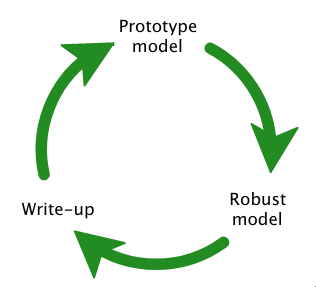
\includegraphics[scale=0.6]{fig/sem-eng.png}
  \caption{Semantics engineering cycle proposed in \cite{popl}}
  \label{fig:sem-eng}
\end{figure}

In this dissertation, we will skip many of the theoretical aspects of Lisp
and Scheme, stopping only at some details on \texttt{amb} and \texttt{call/cc}
and assume the reader can catch most of the syntax on the go.

Without further ado, we will now skim through some features of Scheme and
Racket that we will use throughout the rest of the dissertation. For further
details, the standard references are \cite{sicp} and \cite{r7rs} for Scheme
and \cite{racket} and \cite{htdp} for Racket.

%%%%%%%%%%%%%%%%%%%%%%%%%%%%%%%%%%%%%%%%%%%%%%%%%%%%%%%%%%%%%%%%%%%%%%
\section{Scheme and Racket crash course}

Since both languages emerged from a common ancestor, Lisp, they use (as the
name implies) a \emph{list syntax}. Furthermore, most of the functions
and predicates use a prefix notation and the mathematical operations
use the so-called Polish (\L{}ukasiewicz) notation. Some basic examples, including specific
functions follow.
\begin{itemize}
\item \texttt{(+ (* 5 3) 1)} computes as $ 5 \cdot 3 + 1 $;
\item \texttt{(lambda (x) (rem x 2))} returns a function that computes
  the remainder of its argument modulo 2;
\item \texttt{(cond (a instruction-a) (b instruction-b) (c instruction-c))} is a
  branching conditional expression. If \texttt{a} is true, then \texttt{instruction-a}
  is executed, else if \texttt{b} is true, \texttt{instruction-b} is executed and
  most of the times, \texttt{c} is taken to be \texttt{t} (true) such that the last
  branch is executed if everything else fails.
\end{itemize}

We should remark from the beginning that Racket is almost a superset of Scheme,
and as such, its syntax contains that of Scheme. To be precise, Racket expands
on the standards R5RS (1998) and R6RS (2009) of Scheme, diverging more
significantly from R7RS (2013), but for the purpose of this dissertation, unless
otherwise specified, all Scheme syntax presented is assumed to be valid Racket
syntax.

While it is not typed in the modern sense of the word, Scheme differentiates between
three basic types: \emph{lists}, \emph{functions} and \emph{symbols}, the latter
encompassing \qq{everything else}.

A specific syntax with its corresponding semantics is the \emph{quoting mechanism}.
As such, a \emph{quoted expression}, denoted either by \texttt{(quote (expr))} or
by \texttt{('(expr))} (another valid variation is \texttt{(\#'(expr))}) is one that
evaluates to itself, regardless of what \texttt{expr} contains. In brief, it turns
\texttt{expr} into (a list of) symbols. Examples:
\begin{itemize}
\item \texttt{(lambda (x) '(+ 1 2 3))} is a function that associates to its argument
  the (literal) list \texttt{'(+ 1 2 3)} (notice that the sum is not evaluated, but
  it is returned literally);
\item \texttt{(define animals '(cond cat dog mouse))} defines the variable \texttt{animals}
  to be the (literal) list \texttt{'(cond cat dog mouse)}.\footnote{We are aware that
    there's no \qq{cond} animal, we included it to make it clear that it is not
    evaluated, i.e.\ the list is not seen as a branching conditional, but instead
    returned literally.}
\end{itemize}

The opposite of quoting expressions is \emph{unquoting}, which forces the
evaluation and returns the final value in-place. The syntax for unquoting is
a comma that precedes the expression that is evaluated. Examples:
\begin{itemize}
\item \texttt{(lambda (x) ,(+ 1 2 3))} is a function that returns 6 for all its
  arguments, since it associates to \texttt{x} the \emph{final value} of
  \texttt{(+ 1 2 3)}, which is 6;
\item \texttt{(define sum '(+ 1 2 3)) (define x (* ,sum 2))} makes \texttt{x} to
  be 12, since in its definition, the initially quoted \texttt{sum} is now
  forcibly evaluated.
\end{itemize}

In fact, the unquoting mechanism is an artifice of \emph{metaprogramming}, more
precisely an instance of a macro, which is one of the features that Lisps excel in.

Some more elements of syntax that will provide useful are listed briefly below.

\begin{itemize}
\item As seen above, functions and variables are defined with \texttt{(define ...)}.
  In fact, usually \texttt{define} is used for functions and variables are defined
  and given a value with \texttt{set}. There's also the variation \texttt{set!}, which
  forcibly overwrites whatever value the variable had;
\item \texttt{cons} is the common function for appending to a list;
\item \texttt{car} is the function that returns the head of the list and \texttt{cdr}
  returns its tail, so \texttt{(car '(1 2 3))} evaluates to \texttt{1} and
  \texttt{(cdr '(1 2 3))} evaluates to \texttt{(2 3)};
\item Comments are preceded by semicolons (\texttt{;}) and the convention is to use
  single semicolon for in-line comments and double semicolons for full-line comments.
  Also, in-line comments are used for writing the result of evaluating an expression,
  with an added arrow, e.g.\ \texttt{(+ 2 3) ; => 5}.
\end{itemize}

%%%%%%%%%%%%%%%%%%%%%%%%%%%%%%%%%%%%%%%%%%%%%%%%%%%%%%%%%%%%%%%%%%%%%%
\section{\texttt{amb} and \texttt{call/cc}}

We will now give special attention to \emph{ambiguous evaluation} using the
function \texttt{amb} and also the \emph{continuation} support included
in Scheme, as they are specific features that will be used later on.
Furthermore, from a historical perspective, Lisps were the first to
support both of them. More languages followed, such as:
\begin{itemize}
\item \texttt{amb} implementation in many programming languages is
  comprehensively presented at \cite{rosetta};
\item \emph{continuations} are supported, for example, in Ruby's
  \emph{Continuation} class (\cite{ruby-callcc}), C++'s \emph{context %
    switching} (\cite{callcc-c}) and Haskell's \texttt{Control} monad
  (\cite{haskell-control}).
\end{itemize}

We will only present here the implementation of the two functions in
Scheme, using mostly \cite{sicp} and \cite{nondet}. Furthermore, the
specifications for both are included in \cite{r7rs}. Since \texttt{amb} is
implemented using \texttt{call/cc}, we will start with the latter.

By definition, the \emph{continuation} of a computation is what will happen
after the current computation is performed. For example, in the computation
\texttt{(+ (* 2 3) 5)}, the continuation of the multiplication is the addition
of 5 to the result. As such, one can abstract the continuation from this example
with a lambda expression:
{\small
\begin{verbatim}
(define cont1
  (lambda (x) (+ x 5)))
\end{verbatim}
}
Then, we get the same result as above by calling:
{\small
\begin{verbatim}
(cont1 (* 2 3))     ; => 11
\end{verbatim}
}
While this example may not seem like much, the basic idea that one can capture
\qq{a part} of a computation and reuse it for some other purpose is important.

This concept is captured in the standard \texttt{call/cc} function in Scheme
(sometimes implemented as \texttt{call-with-current-continuation}). Some basic
examples are the following:
{
  \small
\begin{verbatim}
;; Nothing to capture
(define id              ; the identity function
  (lambda (k) k))
(call/cc id)            ; returns the function
                        ; since there's nothing left to do

;; Continuation is just the argument
(define apply-to-zero
  (lambda (k) (k 0)))
(call/cc apply-to-zero) ; returns 0
                        ; since that continues the function

;; Capture a further operation
(+ (call/cc 
     (lambda (k) (k (* 1 2))))
      3)
;; is equivalent to
((lambda (v) (+ v 3)) (* 1 2))

;; Basically, the continuation only is (+ _ 3):
(lambda (x) (+ x 3))
\end{verbatim}
}

The \texttt{call/cc} function can be used for saving a certain point
of a computation. For example, we can save a backup copy of a function
than can be used later:
{
  \small
\begin{verbatim}
(define z #f)                   ; initialize z with false
(+ (call/cc
     (lambda (k)
        (set! z k)              ; clear what's stored in z and put k
        (* 1 2)))
    3)                          ; => 5
\end{verbatim}
}
In the example above, we have stored only the lambda-function in \texttt{z},
so even if the whole computation returns \texttt{5}, we have like a
\qq{bookmark} at the \texttt{lambda} definition which is stored in \texttt{z}.
Henceforth, we can do:
{
  \small
\begin{verbatim}
(z 1)               ; => 4
\end{verbatim}
}

\vspace{0.3cm}

The \texttt{amb} operator is a bit more complicated and although it is
implemented in the standard library in some Scheme distributions, we will
define it manually. We will follow the presentation in \cite{nondet}. This
will define \texttt{amb} as a macro, which ensures that the arguments are not
evaluated and as we will see, it is implemented using \texttt{call/cc}.

The basic idea, as outlined first in \cite{mccarthy61}, is that the \texttt{amb}
operator works as an ambiguous evaluation, with a variable number of arguments,
in the following sense:
\begin{itemize}
\item if none of its arguments can be computed or if no arguments are given,
  it returns some kind of failure (we will use \texttt{\# f} for \texttt{false});
\item if any (one or more) of its arguments can be computed, return all the
  possible values.
\end{itemize}

For example, McCarthy defines in pseudocode:
\[
  \texttt{less(n) = amb(n-1, less(n-1))},
\]
which is a \qq{function} (quotes because it can return multiple values)
that returns all the numbers that are less than the argument \texttt{n}. Thus,
with \texttt{n} assumed to be a positive integer, \texttt{amb} tries to evaluate
both \texttt{n-1} and recursively compute \texttt{less(n-1)}. If both can be computed,
it returns both, which will happen until \texttt{n = 1}, when the final call will be
\texttt{amb(0, less(0))}, that returns \texttt{0} and the computation stops, since
none of the arguments won't work at the next iteration.

Here's how \texttt{amb} can be implemented in Scheme, using \texttt{call/cc}:
{
  \small
\begin{verbatim}
(define f #f)                                       ; 1

(define-syntax amb                                  ; 2
  (syntax-rules ()                                  ; 3
    ((_) (f))                                       ; 4
    ((_ a) a)                                       ; 5
    ((_ a b ...)                                    ; 6
      (let ((s f))                                  ; 7
        (call/cc                                    ; 8
          (lambda (k)                               ; 9
            (set! f (lambda ()                      ; 10
                        (set! f s)                  ; 11
                        (k (amb b ...))))           ; 12
          (k a)))))))                               ; 13
\end{verbatim}
}

The basic ideas are the following:
\begin{itemize}
\item In the \texttt{syntax-rules} declaration, the underscore denotes
  the syntax (function) that is defined, \texttt{amb};
\item The first case (line 4) is when \texttt{amb} is called with no arguments,
  \texttt{(amb)}, case in which it returns \texttt{(f)}, which is \texttt{false};
\item Then, in line 5, if it is called with some argument, it will return that;
\item If it is called with more than one argument (the ellipse being special
  syntax for zero or more arguments that could follow; in a more rigorous setting,
  it is in fact a \emph{Kleene star}), then the actual work is done:
  \begin{itemize}
  \item first, we introduce a variable \texttt{s} and bind it to \texttt{f}, which is
    \texttt{false};
  \item then, \texttt{call/cc} is called to capture the current continuation in \texttt{k};
  \item inside this \texttt{lambda}, \texttt{f} is reset and a recursive call is made,
    invoking \texttt{k} (the previous computation) to \texttt{amb} called with the rest
    of the arguments (starting with \texttt{b});
  \item finally, in line 13, the captured outermost \texttt{lambda} is applied to \texttt{a},
    which makes the innermost \texttt{lambda} be called only after this computation, so
    first it tries to compute \texttt{(amb a)}
  \end{itemize}
\end{itemize}

\begin{remark}\label{rk:first-res}
  Note that by default, many Scheme and Racket implementations make \texttt{amb}
  behave step by step. That is, when called with multiple arguments, of which more
  than one can be computed, the first evaluation returns only the first computation.
  Calling \texttt{amb} again returns the second possible computation etc.
  Hence, for example, Racket 7.5 REPL, using the \texttt{\#lang scheme} pragma,
  gives the following session, using the implementation above:
  {
    \small
\begin{verbatim}
REPL> (amb "dog" "cat")
"dog"
REPL> (amb)
"cat"
REPL> (amb)
#f
\end{verbatim}
  }
\end{remark}

\vspace{0.3cm}

\begin{remark}\label{rk:resources}
  One last word regarding the source code and the entire contents of this
  dissertation. While Racket comes with an exceptionally powerful and user-friendly
  IDE called \texttt{DrRacket} which is automatically installed when installing
  the language and for which the book \cite{htdp} can be seen as an extensive
  user manual, we have chosen to write and test everything contained in this
  dissertation in GNU Emacs 26.3 running under Manjaro Linux. Scheme support is
  built in and for Racket, we used the full-featured REPL included in
  \href{https://www.racket-mode.com/}{racket-mode}.
\end{remark}

%%% Local Variables:
%%% mode: latex
%%% TeX-master: "../redex"
%%% End:
